\section{Descoberta Causal}

\begin{frame}{Descoberta Causal}
    \texttt{Causal Discovery (CD)} é o processo de aprender estruturas causais a partir de dados observacionais, sem depender de conhecimento de negócio (nem sempre é possível realizar experimentos).

    A partir de dados observacionais, o objetivo é inferir um grafo causal (ou classe de equivalência) que represente as relações causais.

    \begin{figure}
        \centering
        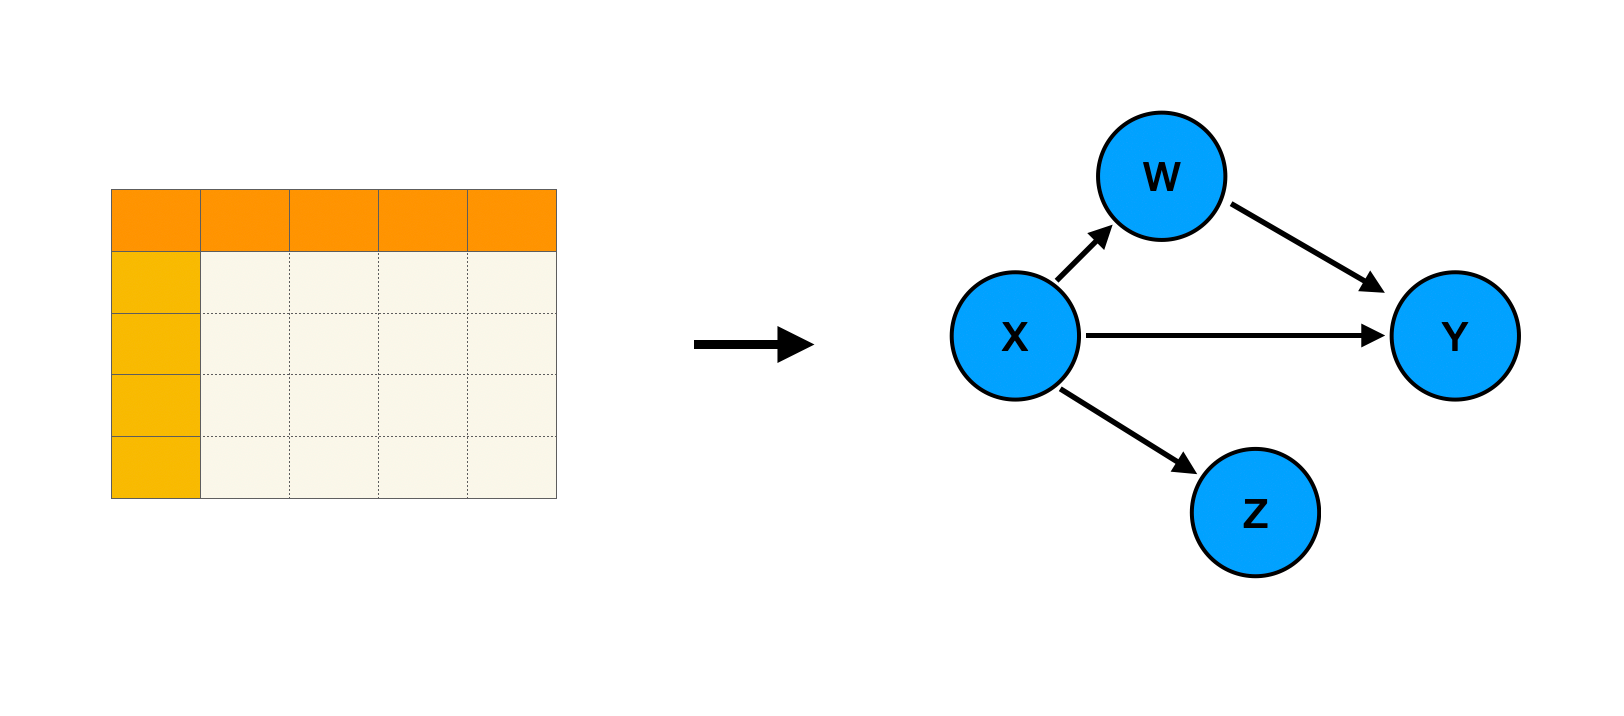
\includegraphics[width=0.75\textwidth]{figures/causal_discovery.png}
    \end{figure}
\end{frame}

\begin{frame}{Descoberta Causal}
    Dados observacionais sozinhos geralmente identifica apenas a classe de equivalência representado por um \textit{CPDAG} (Completed Partially Directed Acyclic Graph) e não um único DAG.

    \pause

    O problema é muito desafiador por diversos motivos:
    \begin{itemize}
        \item O espaço de busca de possíveis grafos cresce super-exponencialmente com o número de variáveis;
        \pause
        \item Amostras finitas podem fornecer estimativas não confiáveis de independências condicionais;
        \pause
        \item A presença de variáveis latentes (não observadas) pode impedir que a verdadeira estrutura seja identificada apenas com dados.
    \end{itemize}
\end{frame}

\begin{frame}{Descoberta Causal}{Famílias de abordagens}
    \begin{itemize}
        \item \textbf{Constraint-based}: Utiliza testes de independência condicional para inferir a estrutura causal. Exemplo: PC, FCI.
        \pause
        \item \textbf{Score-based}: Busca por uma estrutura que maximize uma função de pontuação (score) equilibrando fit e complexidade. Exemplo: GES, BIC.
        \pause
        \item \textbf{Functional}: Explora assimetrias na forma funcional de relações entre variáveis para inferir causalidade. Exemplo: LiNGAM, ANM. - Assumem relações lineares e sem ruído gaussiano, podendo identificar até um DAG completo, se as premissas forem atendidas.
        \pause
        \item \textbf{Hybrid}: Combina elementos de diferentes abordagens.
    \end{itemize}
\end{frame}

\begin{frame}{Descoberta Causal}{Escolhendo um algoritmo de CD}
    \begin{columns}[T]
        \begin{column}{0.25\textwidth}
            \begin{figure}
                \centering
                
\includegraphics[width=0.9\textwidth]{figures/choice_guy.jpg}
            \end{figure}
        \end{column}
        \begin{column}{0.75\textwidth}
            Escolher um algoritmo de CD depende de características como:
            \begin{itemize}
                \item Tamanho do conjunto de dados (número de amostras e variáveis);
                \pause
                \item Premissas sobre a distribuição dos dados (linearidade, ruído, etc.);
                \pause
                \item Tipos de dados suportados (contínuos, discretos);
                \pause
                \item Robustez a ruído e outliers.
            \end{itemize}
            \pause
            Não existe bala de prata. \\ Na prática, é comum testar vários e buscar um consenso ou utilizar conhecimento de negócio para validar os resultados.
        \end{column}
    \end{columns}
\end{frame}

\begin{frame}[plain]
    \begin{table}[htbp]
    \centering
    \label{tab:discovery_algorithms}
    \footnotesize
    \begin{tabular}{llccc}
    \toprule
    \textbf{Algorithm} & \textbf{Full Name} & \makecell{\textbf{Supported} \\ \textbf{Data Types}} & \makecell{\textbf{Gaussian} \\ \textbf{Assumption}} & \textbf{Family} \\
    \midrule
    PC \cite{discovery-pc} & Peter-Clark & C, D & No & Constraint \\
    GS \cite{discovery-gs} & Grow-Shrink & C, D & No & Constraint \\
    IAMB \cite{discovery-iamb} & Incremental Assoc. Markov Blanket & C, D & No & Constraint \\
    Fast-IAMB \cite{discovery-iamb-variants} & Fast Markov Blanket & C, D & No & Constraint \\
    Inter-IAMB \cite{discovery-iamb-variants} & Interleaved Markov Blanket & C, D & No & Constraint \\
    MMPC \cite{discovery-mmpc} & Max-Min Parents and Children & C, D & No & Constraint \\
    \midrule
    GES \cite{discovery-ges} & Greedy Equivalence Search & C, D & Yes & Score \\
    GIES \cite{discovery-ges_gies} & Greedy Interv. Equivalence Search & C, D & Yes & Score \\
    CCDr \cite{discovery-ccdr} & Concave penalized Coord. Descent & C & Yes & Score \\
    BES \cite{discovery-bes} & Bayesian Equivalence Search & C, D & Yes & Score \\
    CGNN \cite{discovery-cgnn} & Causal Generative Neural Networks & C & No & Score \\
    SAM \cite{discovery-sam} & Structural Agnostic Model & C & No & Score \\
    \midrule
    LiNGAM \cite{discovery-lingam} & Linear Non-Gaussian Acyclic Model & C & No\textsuperscript{*} & Functional \\
    CAM \cite{discovery-cam} & Causal Additive Models & C & Yes & Functional \\
    \midrule
    GRaSP \cite{discovery-grasp} & Greedy Relax. of Sparsest Perm. & C, D & No & Hybrid \\
    \bottomrule
    \multicolumn{5}{l}{\scriptsize \textsuperscript{*}LiNGAM assumes linear relationships with non-Gaussian noise.}
    \end{tabular}
    \end{table}
\end{frame}

\begin{frame}{Mão na massa}
	\notebooklink{2}{2\_causal\_discovery.ipynb}
\end{frame}
